\chapter{门控循环单元(GRU)流变学本构方程建模研究}
% 3.2表================================================
% % 本节仅展示使用常见的三线表
% \begin{table}
%   \TableBicaption{\label{TDF_para}涵道模型参数}{Parameters of Ducted Fan Model}  % 中英文标题
%   \centering
%   \small
%   \begin{tabularx}{\textwidth}{XXXX}  % 使用 tabularx 环境,均匀分布列宽
%     \Xhline{1.5pt}
%     参数符号       & 数值                 & 参数符号  & 数值                 \tabularnewline
%     \Xhline{0.5pt}  % 表头下方线
%     $I_x$      & $054593$           & $I_y$ & $0.017045         $ \tabularnewline
%     $l_1$      & $0.0808\,\text{m}$ & $l_2$ & $0.175\,\text{m}  $ \tabularnewline
%     $l_4$      & $0.2415\,\text{m}$ & $l_5$ & $0.1085\,\text{m} $ \tabularnewline
%     $l_\sigma$ & $xdf$              & $df$  & 扫描电镜 \tabularnewline
%     \Xhline{1.5pt}
%   \end{tabularx}
% \end{table}
\section{引言}
近年来,深度学习在流变学本构建模研究中得到广泛应用。例如Lennon、Mahmoudabadbozchelou等人的研究工作,虽然具体方法各有不同,但在模型选择上基本都采用了多层感知机模型(Multi-Layer Perceptron,MLP)\cite{lennonScientificMachineLearning2023a,mahmoudabadbozchelouDatadrivenPhysicsinformedConstitutive2021}。MLP是一种经典的前馈人工神经网络,由输入层、多个隐藏层及输出层的全连接层堆叠而成,通过非线性激活函数实现复杂函数逼近。当MLP的隐藏层数达到一定值时,它被视为深度神经网络(Deep Neural Network,DNN)。传统的前馈性质DNN模型虽具备一定的非线性行为捕捉能力,但在处理具有时间依赖性的数据时,其性能往往受到限制。Lennon和Mahmoudabadbozchelou的工作使用DNN模型,难以有效捕捉黏弹性材料中的长程应变历史依赖性。本章研究在前人基础上,采用门控循环单元(Gated Recurrent Unit,GRU)进行本构建模,旨在解决DNN模型在处理时间序列数据时性能受限的问题。GRU的门控机制能够在处理流变学数据(如应力应变数据)时,有效控制历史信息在网络中的流动。

本章研究首先通过数值模拟方法构建了多种经典本构方程的应力应变数据,包括Herschel-Bulkley模型、Maxwell模型和Doi-Edwards模型。这些模型在流变学领域具有重要的理论和应用价值,能够描述不同类型的流变行为。随后,本章详细设计了GRU模型的结构、参数初始化及训练优化策略,并使用数值模拟生成的应力应变数据进行训练和参数优化,使模型能够准确拟合训练数据。为了验证GRU模型在探索未知流变学本构方程方面的能力,本章将训练好的GRU模型应用于未经训练的测试集数据,并通过与经典DNN模型的对比,验证了GRU模型在处理时间序列数据方面的优势。

\section{算法介绍}
\subsection{时间序列数据介绍}
时间序列数据是指在一系列时间点上按时间顺序排列的数据点集合。这些数据点通常是连续或定期记录的,反映了某个变量随时间的变化情况。在流变学研究中,时间域的应力应变数据在小应变时满足玻尔兹曼叠加原理,即当前应力状态为之前所有应变历史的线性和\cite{boltzmannZurTheorieElastischen1878}。大应变时应力应变数据虽然不满足玻尔兹曼的线性叠加,但是依旧可以表示为过去应变历史的非线性关系叠加。

\subsection{循环神经网络}
\subsubsection{简单RNN}
循环神经网络(Recurrent Neural Network,RNN)是一种专门处理序列数据的神经网络结构,其核心在于利用循环结构捕捉时间或顺序上的依赖关系\cite{elmanFindingStructureTime1990}。RNN的基本结构由输入层、隐藏层和输出层组成(图\ref{rnn_gru illustration}(a))。隐藏层中的神经元不仅接收来自输入层的信号,还接收来自前一时刻隐藏层的信号。这种循环连接使得RNN能够捕获序列中的时间依赖关系。
RNN的数学模型可以通过公式\eqref{eq:rnnht}描述:
\begin{align}
   & \mathbf{h}_t = \sigma(\mathbf{W}_{xh} \mathbf{x}_t + \mathbf{W}_{hh} \mathbf{h}_{t-1} + \mathbf{b}_h) \label{eq:rnnht} \\
   & {\mathbf{o}_t = \mathbf{W}_{ho} \mathbf{h}_t + \mathbf{b}_o} \label{eq:rnnot}
\end{align}
其中$\mathbf{h}_t$ 是时刻 $t$ 的隐藏状态,$\mathbf{x}_t$ 是时刻 $t$ 的输入,$\mathbf{o}_t$ 是时刻 $t$ 的输出,$\mathbf{W}_{xh}$ 是输入到隐藏层的权重矩阵,$\mathbf{W}_{hh}$ 是隐藏层到隐藏层的权重矩阵,$\mathbf{W}_{ho}$ 是隐藏层到输出层的权重矩阵,$\mathbf{b}_h$ 和 $\mathbf{b}_o$ 是偏置。$\sigma$是激活函数,通常使用 $\tanh$ 或 $\text{ReLU}$。RNN 的训练过程通常使用反向传播算法。通过计算梯度来更新权重矩阵,从而最小化损失函数。

在简单的RNN中,存在梯度消失问题,这主要源于反向传播过程中梯度的连乘效应\cite{schmidhuber1997long}。损失函数 $L$ 对 $\mathbf{W}_{hh}$ 的梯度可以表示为公式\eqref{eq:rnngradient}:
\begin{align}
  \frac{\partial L}{\partial \mathbf{W}_{hh}} = \sum_{t=1}^{T} \frac{\partial L}{\partial \mathbf{h}_t} \cdot \frac{\partial \mathbf{h}_t}{\partial \mathbf{W}_{hh}} \label{eq:rnngradient}
\end{align}
展开后,隐藏状态关于$\mathbf{W}_{hh}$ 的导数为公式\eqref{eq:rnngradient2}:
\begin{align}
  \frac{\partial \mathbf{h}_t}{\partial \mathbf{W}_{hh}} = \sigma'(\mathbf{W}_{hh} \mathbf{h}_{t-1} + \mathbf{W}_{xh} \mathbf{x}_t + \mathbf{b}_h) \cdot \mathbf{h}_{t-1}^T \label{eq:rnngradient2}
\end{align}
注意到,$\frac{\partial L}{\partial \mathbf{h}_t}$依赖于前一个时间步的梯度,如公式\eqref{eq:rnngradient3}:
\begin{align}
  \frac{\partial L}{\partial \mathbf{h}_t} = \frac{\partial L}{\partial \mathbf{h}_{t+1}} \cdot \frac{\partial \mathbf{h}_{t+1}}{\partial \mathbf{h}_t} = \frac{\partial L}{\partial \mathbf{h}_{t+1}} \cdot \mathbf{W}_{hh} \cdot \sigma'(\mathbf{h}_t) \label{eq:rnngradient3}
\end{align}
这表明梯度在通过时间反向传播时会乘以$\mathbf{W}_{hh}$。
从时间$t$到时间$T$的梯度可以表示为公式\eqref{eq:rnngradient4}:
\begin{align}
  \frac{\partial L}{\partial \mathbf{h}_t} = \left( \prod_{k=t+1}^{T} \mathbf{W}_{hh} \cdot \sigma'(\mathbf{h}_{k-1}) \right) \cdot \frac{\partial L}{\partial \mathbf{h}_T} \label{eq:rnngradient4}
\end{align}
其中乘积 $\prod_{k=t+1}^{T} \mathbf{W}_{hh} \cdot \sigma'(\mathbf{h}_{k-1})$在某些情况下可能会非常小,例如如果 $\mathbf{W}_{hh}$的特征值小于1,那么随着$(T - t)$的增加,$\mathbf{W}_{hh}^{T-t}$将呈指数级减小并趋近于零。
如果反向传播过程中每一项都小于1,那么整个乘积将随着 $(T - t)$的增加呈指数级减小。
这意味着对于远离输出端的时间步$t$,梯度$\frac{\partial L}{\partial \mathbf{h}_t}$将非常小,导致权重更新几乎停止,这就是RNN的梯度消失问题。由于RNN为了捕捉时间依赖性,我们不可避免地设置长时间步,这导致RNN梯度消失问题几乎难以避免。
\subsubsection{GRU}
为了解决简单RNN的梯度消失问题,Schmidhuber等提出了长短期记忆网络(Long Short-Term Memory,LSTM)\cite{schmidhuber1997long}。LSTM通过引入门控机制来控制信息的流动,从而有效地缓解梯度消失问题。LSTM的核心结构包括输入门、遗忘门和输出门,这些门控机制能够有效地控制信息的流动,从而捕获长期依赖关系。

LSTM虽然通过引入门控机制有效地解决了简单RNN中的梯度消失问题,但在实际应用中仍然存在一些问题。LSTM包含三个门(输入门、遗忘门、输出门),导致其参数数量较多,增加了模型的复杂度和计算成本。由于LSTM的复杂结构,其训练和推理速度相对较慢,尤其是在处理大规模数据时。为了解决LSTM的上述问题,Cho等提出了GRU作为LSTM的简化版本\cite{choLearningPhraseRepresentations2014}(图\ref{rnn_gru illustration}(b))。GRU的设计初衷是为了简化LSTM的结构,同时保持其捕获长期依赖关系的能力。GRU只有重置门(Reset Gate)和更新门(Update Gate)两种门控单元,与LSTM相比,GRU的参数数量较少,训练和推理速度更快。重置门的计算公式为公式\eqref{eq:grureset}。
\begin{align}
  \mathbf{r}_t = \sigma(\mathbf{W}_r \mathbf{x}_t + \mathbf{U}_r \mathbf{h}_{t-1} + \mathbf{b}_r) \label{eq:grureset}
\end{align}
更新门的计算公式为公式\eqref{eq:gruupdate},重置门决定了前一时间步的隐藏状态在多大程度上被忽略。当重置门的输出接近0时,网络倾向于“忘记”前一时间步的信息,仅依赖于当前输入;而当输出接近1时,前一时间步的信息将被更多地保留。
更新门决定了多少过去的信息将被保留,而新信息将占据多少比例。当更新门的输出接近1时,新的隐藏状态几乎等同于旧的隐藏状态,从而实现了长期依赖的捕捉;当更新门的输出接近0时,新的隐藏状态将主要由当前输入决定。
\begin{figure}[htbp]
  \centering
  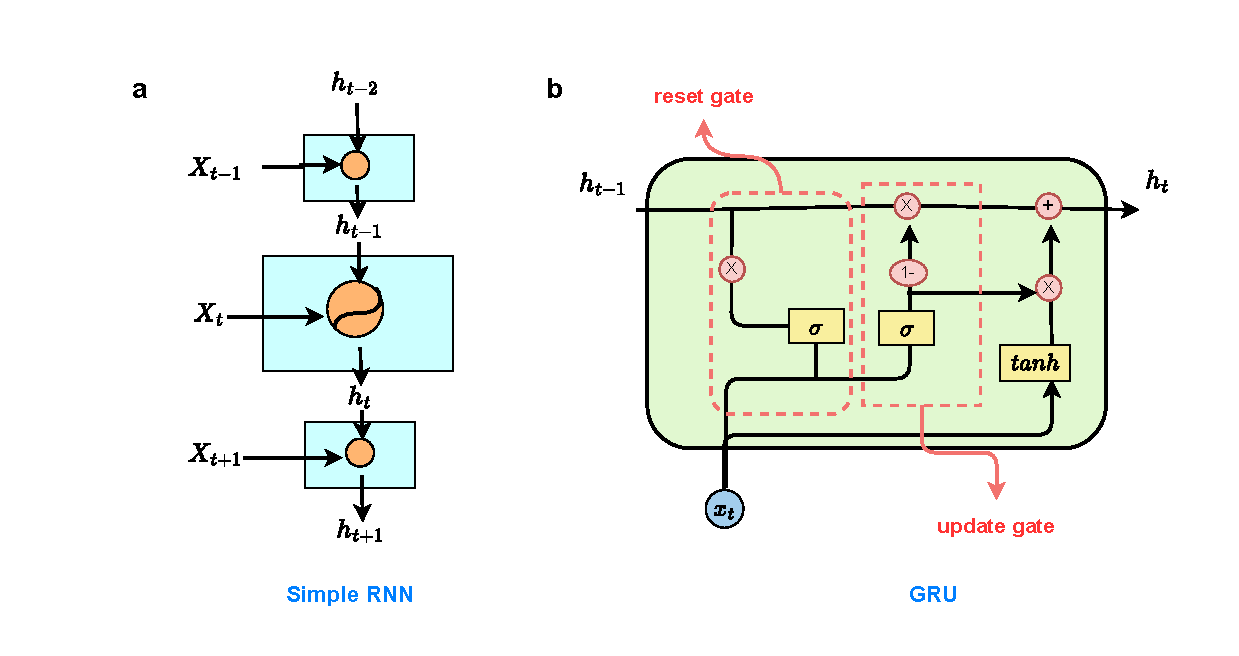
\includegraphics[width=0.9\textwidth]{Fig/rnn-gru.pdf}
  \FigureBicaption{\label{rnn_gru illustration}(a)RNN 示意图 ;(b)GRU 示意图}{Schematic illustration of (a) RNN and (b) GRU}
\end{figure}
\begin{align}
  \mathbf{z}_t = \sigma(\mathbf{W}_z \mathbf{x}_t + \mathbf{U}_z \mathbf{h}_{t-1} + \mathbf{b}_z) \label{eq:gruupdate}
\end{align}
候选隐藏状态决定了当前时间步的新信息,如公式\eqref{eq:gruhih}所示。
\begin{align}
  \tilde{\mathbf{h}}_t = \tanh(\mathbf{W}_h \mathbf{x}_t + \mathbf{U}_h (\mathbf{r}_t \odot \mathbf{h}_{t-1}) + \mathbf{b}_h) \label{eq:gruhih}
\end{align}
当前隐藏状态如公式\eqref{eq:gruhi}所示,这里的当前隐藏状态与上文LSTM的隐藏状态含义是一样的。
\begin{align}
  \mathbf{h}_t = (1 - \mathbf{z}_t) \odot \mathbf{h}_{t-1} + \mathbf{z}_t \odot \tilde{\mathbf{h}}_t \label{eq:gruhi}
\end{align}

GRU移除了单元状态的概念,直接从门控单元来计算隐藏状态,GRU 通过重置门和更新门的协同工作,实现了对信息流动的有效控制,使得网络能够在需要时记住长期依赖关系,同时减少梯度消失/爆炸的问题。GRU的结构比LSTM更简单,计算效率更高,因此在实践应用中广受欢迎。本章使用GRU模型进行流变学本构方程的预测建模。

\section{实验设计}
\subsection{数据获取}
\subsubsection{Herschel-Bulkley模型模拟数据}
Herschel-Bulkley模型的本构方程如公式\eqref{eq:herschel}所示,其中剪切应力$\sigma$与剪切率$\dot{\gamma}$之间存在函数关系。该模型包含流变参数$K$、流动指数$n$及屈服应力$\sigma_0$。在模拟过程中,本章设置$\sigma_0$为1.0 Pa,$K$为1,而$n$则取值为0.2、0.6、1.0、1.4及1.8。剪切率$\dot{\gamma}$范围设定为[0,100],并以0.01的时间步长进行离散采样。

数据生成后,本章首先采用Matplotlib库绘制出剪切应力$\sigma$与剪切率$\dot{\gamma}$的关系曲线,观察模拟效果,并进行生成效果评估。随后本章采用NumPy库进行数据处理,使用Pandas库将数据存储为Excel文件,便于后续的模型训练。
\subsubsection{Maxwell模型模拟数据}
Maxwell模型的微分本构方程如公式\eqref{eq:maxwell_model_dt}所示。该模型包含松弛时间$\tau=\eta/G$,其中$\eta$表示黏性系数,$G$为剪切模量。本章设置$\eta$为0.1 Pa·s,$G$为1.0 Pa。采用后向欧拉法来离散化微分方程,具体推导如下:

首先将微分离散化,设$d\sigma=\sigma_i - \sigma_{i-1}$,$dt=\Delta t$,$d\gamma=\gamma_i - \gamma_{i-1}$,则原方程可以化简为公式\eqref{eq:maxwell_euler_back_1},
\begin{equation}
  \frac{\sigma_i - \sigma_{i-1}}{\Delta t} + \frac{\sigma_i}{\tau} = G \frac{\gamma_i - \gamma_{i-1}}{\Delta t} \label{eq:maxwell_euler_back_1}
\end{equation}
移项并化简可得公式\eqref{eq:maxwell_euler_back_2}。
\begin{equation}
  \sigma_i = \frac{\sigma_{i-1} + G (\gamma_i - \gamma_{i-1})}{1 + \frac{\Delta t}{\tau}} \label{eq:maxwell_euler_back_2}
\end{equation}
根据公式\eqref{eq:maxwell_euler_back_2},本章首先使用NumPy库生成6个不同应变变化协议的应变数据,时间步为0.01 s,每个协议模拟2000个数据点,并存为NumPy数组,随后通过迭代法计算单个应变数据对应的应力数据,并存为NumPy数组。之后,本章使用Matplotlib库绘制出剪切应力与剪切应变的关系曲线,观察模拟效果,并进行生成效果评估。最后本章使用Pandas库将数据存储为Excel文件,便于后续的模型训练。
\subsubsection{Doi-Edwards模型模拟数据}
Doi-Edwards模型的本构方程如公式\eqref{eq:doi_edwards}所示。该方程为积分形式的本构方程,本章首先对该方程进行处理,将取向张量函数$\mathbf{Q}(t^{\prime},t)$写为球坐标形式,即公式\eqref{eq:doi_edwards_moni_q}。
\begin{align}
   & \mathbf{Q}(t^{\prime},t) = \frac{1}{4\pi} \int_{0}^{2\pi} \int_{0}^{\pi} 5 \left( \frac{\mathbf{u}^{\prime} \cdot \mathbf{F}^{-1} \mathbf{u}^{\prime} \cdot \mathbf{F}^{-1}}{|\mathbf{u}^{\prime} \cdot \mathbf{F}^{-1}|^{2}} \right) \sin\theta \, d\theta \, d\phi   \label{eq:doi_edwards_moni_q} \\
   & G(t, t') = \frac{G_0}{\lambda_i} \exp\left( \frac{t' - t}{\lambda_i} \right)   \label{eq:doi_edwards_moni_g}                                                                                                                                                                                         \\
   & \boldsymbol{\sigma}(t) = \int_{t_0}^t G(t, t') \cdot \mathbf{Q}(\gamma(t')) \, dt' \label{eq:doi_edwards_moni_sigma}
\end{align}

本章模拟的为简单剪切流动,只在xy方向存在应变,因此可以将逆变形梯度张量$\mathbf{F}^{-1}$写为公式\eqref{eq:doi_edwards_f_inverse}的矩阵形式,$\mathbf{u}^{\prime}$为球坐标系下的单位向量。
\begin{equation}
  \mathbf{F}^{-1} = \begin{bmatrix}
    1      & 0 & 0 \\
    \gamma & 1 & 0 \\
    0      & 0 & 1
  \end{bmatrix} \label{eq:doi_edwards_f_inverse}
\end{equation}
公式\eqref{eq:doi_edwards_moni_g}为松弛模量函数,本章使用NumPy库生成7个不同的应变协议的NumPy数组,单个协议时间区间为[0,4$\pi$],总数据点为2000个,生成形式为3$\times$3的张量矩阵,代入公式\eqref{eq:doi_edwards_moni_q}计算$\mathbf{Q}$值数组。设置$G_0$为1.0 Pa,$\lambda$为1.0 s,$i=1$,根据公式\eqref{eq:doi_edwards_moni_sigma}计算应变张量,使用的积分工具为Python的scipy.integrate库,生成形式为3$\times$3的张量矩阵,如公式\eqref{eq:sigma_bmatrix}所示。本章提取$
  \sigma_{12}$、$\sigma_{11}$、$\sigma_{22}$分量作为模拟实验数据,与对应的应变分量数据一起通过Pandas库存入Excel文件,便于后续的模型训练。
\begin{equation}
  \boldsymbol{\sigma} = \begin{bmatrix}
    \sigma_{11} & \sigma_{12} & \sigma_{13} \\
    \sigma_{21} & \sigma_{22} & \sigma_{23} \\
    \sigma_{31} & \sigma_{32} & \sigma_{33}
  \end{bmatrix} \label{eq:sigma_bmatrix}
\end{equation}

\subsection{模型训练}
\subsubsection{数据集划分}
首先本章对模拟生成的数据进行数据集划分,将数据集分为训练集(Train)、验证集(Valid)和测试集(Test),不同模型的具体划分如下:

Herschel-Bulkley模型数据单独划分$n=1.0$的数据为测试集,其余数据按照9:1比例划分为训练集和验证集。

Maxwell模型数据单独划分4个交变应变协议为训练集和验证集,其中按照9:1比例划分为训练集和验证集。划分1个交变应变协议,1个线性应变协议为测试集。

Doi-Edwards模型数据单独划分5个交变应变协议为训练集和验证集,其中按照9:1比例划分为训练集和验证集。划分1个交变应变协议,1个线性应变协议为测试集。

\subsubsection{损失函数构建}
本章构建的损失函数主要包括均方误差(Mean Squared Error,MSE)损失和L$_2$正则化损失两部分。均方误差损失用于衡量模型预测值与真实值之间的差异,L$_2$正则化损失则用于防止模型过拟合。

均方误差损失函数的数学表达式如公式\eqref{eq:mse_loss}所示:
\begin{equation}
  \mathcal{L}_{\text{MSE}} = \frac{1}{n} \sum_{i=1}^{n} (y_i - \hat{y}_i)^2 \label{eq:mse_loss}
\end{equation}
其中,$y_i$表示第$i$个样本的真实值,$\hat{y}_i$表示模型对第$i$个样本的预测值,$n$表示样本总数。MSE损失函数对误差进行平方处理,使得较大的误差在优化过程中受到更多关注,有利于模型快速收敛到最优解。

L$_2$正则化损失函数的数学表达式如公式\eqref{eq:l1_loss}所示:
\begin{equation}
  \mathcal{L}_{\text{L$_2$}} = \lambda \sum_{j=1}^{m} |\theta_j| \label{eq:l1_loss}
\end{equation}
其中,$\theta_j$表示模型的第$j$个参数,$m$表示模型参数总数,$\lambda$为正则化系数,用于控制正则化强度。L$_2$正则化通过惩罚较大的参数值,促使模型学习更加平滑的函数,从而提高模型的泛化能力。

综合以上两部分,本章采用的总损失函数如公式\eqref{eq:total_loss}所示:
\begin{equation}
  \mathcal{L}_{\text{total}} = \mathcal{L}_{\text{MSE}} + \mathcal{L}_{\text{L$_2$}} = \frac{1}{n} \sum_{i=1}^{n} (y_i - \hat{y}_i)^2 + \lambda \sum_{j=1}^{m} \theta_j^2 \label{eq:total_loss}
\end{equation}

\subsubsection{训练细节}
本章的模型训练流程相同。首先对数据集进行划分,接着对训练集和验证集的数据实施归一化处理,随后将其转换为 Torch 张量。利用 Pytorch 框架编写模型代码,开展深度学习训练。在训练期间,采用 Adam 优化算法,以 MSE 损失函数为评估标准,借助网格搜索算法和随机搜索算法实现超参数的优化与选择。待训练结束后,把模型参数存储为 .pth 文件,方便后续进行模型测试。

\subsection{模型测试}
\subsubsection{测试指标细节}
本章的模型训练均为回归问题,所以采用的测试指标为决定系数(Coefficient of Determination,R$^2$),如公式\eqref{eq:r2}所示,平均绝对误差(Mean Absolute Error,MAE),如公式\eqref{eq:mae}所示,平均百分比误差(Mean Absolute Percentage Error,MAPE),如公式\eqref{eq:mape}所示。
\begin{equation}
  \text{R}^2 = 1 - \frac{\sum_{i=1}^{n} (y_i - \hat{y}_i)^2}{\sum_{i=1}^{n} (y_i - \bar{y})^2} \label{eq:r2}
\end{equation}
\begin{equation}
  \text{MAE} = \frac{1}{n} \sum_{i=1}^{n} |y_i - \hat{y}_i| \label{eq:mae}
\end{equation}
\begin{equation}
  \text{MAPE} = \frac{100\%}{n} \sum_{i=1}^{n} \left| \frac{y_i - \hat{y}_i}{y_i} \right| \label{eq:mape}
\end{equation}
此外,加上训练时间作为训练成本指标。

\subsubsection{测试实验划分}
Herschel-Bulkley模型使用训练后保存的模型参数,使用测试集时间进行预测,训练数据与测试数据为不同的流动指数$n$,采用已知流动指数数据预测未知流动指数数据,预测物理量为剪切应力。按照上述实验步骤分别使用DNN和GRU两种模型进行测试,绘制两个模型的测试比对曲线。

Maxwell模型训练数据为交变应变数据,其应变关系符合公式\eqref{eq:sin_gamma_protocol},测试数据分为交变应变数据和公式\eqref{eq:linear_gamma_protocol}所示的稳态应变数据。采用已知交变协议数据预测未知交变协议数据,已知交变协议数据预测未知稳态协议数据,预测物理量为剪切应力。按照上述实验步骤分别使用DNN和GRU两种模型进行测试,绘制两个模型的测试比对曲线。对于GRU模型,设置不同的序列时间步进行训练,探究模型的最佳时间步。
\begin{equation}
  \gamma=\gamma_0cos(\omega t+\phi) \label{eq:sin_gamma_protocol}
\end{equation}
\begin{equation}
  \gamma=\dot{\gamma}t \label{eq:linear_gamma_protocol}
\end{equation}

Doi-Edwards模型与Maxwell模型的实验流程一致,采用已知交变协议数据预测未知交变协议数据,已知交变协议数据预测未知线性协议数据,预测物理量为xy方向剪切应力$\sigma_{12}$和第一法向应力差$N_1$。第一法向应力差的公式为$N_1=\sigma_{11}-\sigma_{12} $,其中$\sigma_{11}$和$\sigma_{22}$ 分别表示xx方向和yy方向的应力。按照上述实验步骤分别使用DNN和GRU两种模型进行测试,绘制两个模型的测试比对曲线。对于GRU模型,设置不同的序列时间步进行训练,探究模型的最佳时间步。

\section{结果与讨论}
\subsection{Herschel-Bulkley模型建模}
\subsubsection{数值模拟数据}
\begin{figure}[htbp]
  \centering
  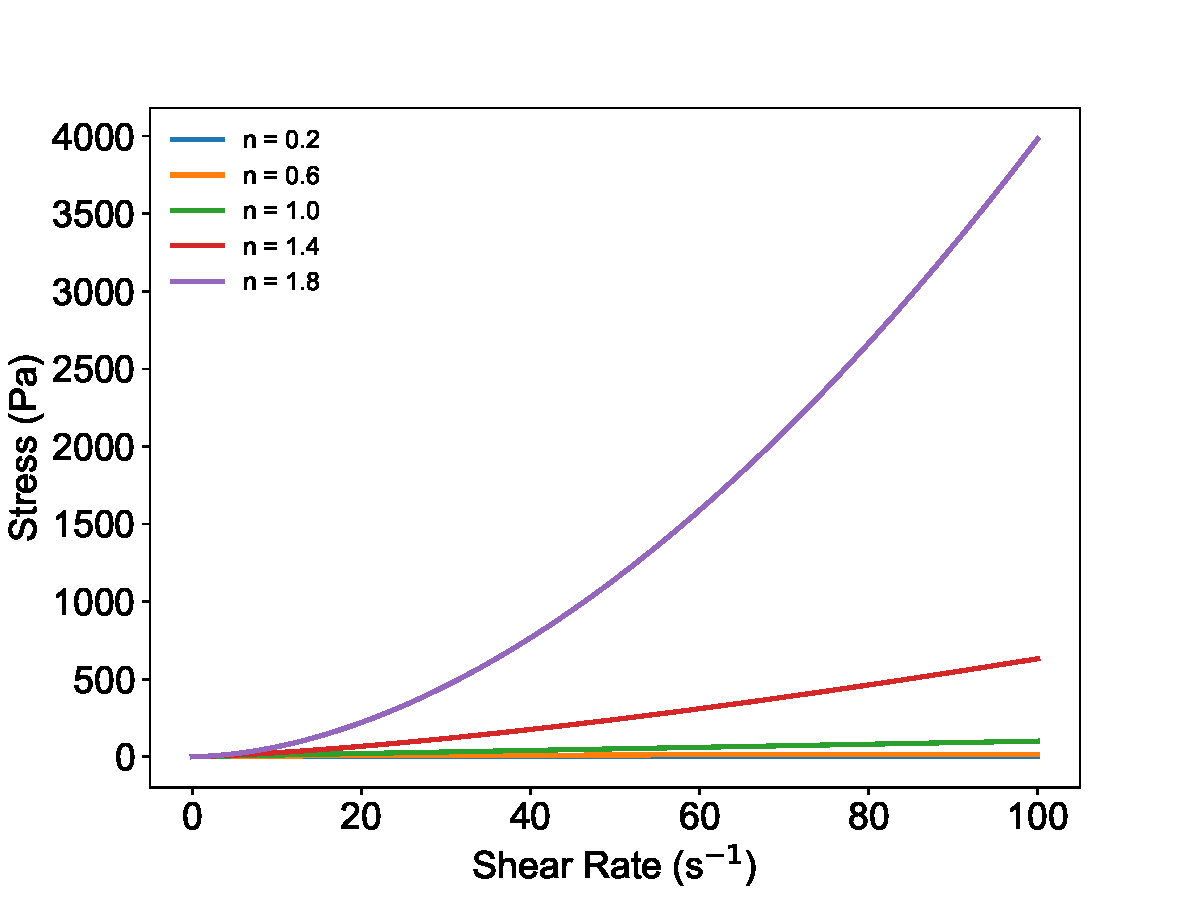
\includegraphics[width=0.8\textwidth]{Fig/herschel_moni.pdf}
  \FigureBicaption{\label{herschel_moni}Herschel-Bulkley模型模拟数据应力-应变率曲线图,n为流变指数}{Stress–strain rate curve of simulated data for the Herschel-Bulkley model, where n represents the flow index}
\end{figure}
本节使用Herschel-Bulkley模型模拟数据,模拟结果如图\ref{herschel_moni}所示。由图\ref{herschel_moni}可以看到,模拟数据中剪切应力Stress与剪切速率Shear Rate呈现幂函数关系,随着流变指数$n$的增加,曲线的斜率增大,表明流体的非牛顿特性增强。这一现象与Herschel-Bulkley模型的数学形式相符,说明模拟数据符合预期。
\subsubsection{GRU/DNN模型预测效果对比}

本节分别使用GRU和DNN两种算法对Herschel-Bulkley模型模拟数据进行深度学习建模,之后使用预测模型在测试集上进行验证,测试结果如图\ref{herschel_test}所示。图\ref{herschel_test}(a)为两种算法测试的真实值-预测值曲线,从曲线可以定性看出两种算法的预测值曲线与真实值曲线都非常接近。图\ref{herschel_test}(b)为两种算法测试结果的残差图,可以看出两种算法的残差点离散程度接近,均没有明显趋向性,均呈现无序分布,说明两种算法均可以比较好地捕捉到所有的输入特征。图\ref{herschel_test}(c-f)分别比较了两种算法预测结果的R$^2$,MAE,MAPE指标,从结果中可以看出,两种算法的预测效果都十分良好,R$^2$都接近1,GRU预测结果的R$^2$值略高于DNN,GRU预测结果的MAE和MAPE值都小于DNN,但数值差距不大。GRU算法的平均训练时间为378 s,高于DNN的155 s 一倍以上,这是由于GRU网络的参数量更大,且由于其循环神经网络的特点,只能顺序运算,限制了GPU的并行计算能力,导致训练时间较长。

综合看来GRU和DNN两种算法在Herschel-Bulkley模型模拟数据上的预测表现比较接近,从预测指标的绝对数值看,GRU略优于DNN。这个结果符合预期,因为Herschel-Bulkley模型本质上是模拟了剪切稀化增稠过程,不涉及黏弹性材料的时间依赖性,并且我们模拟的过程中,对于某个特定时间的应力状态也仅仅是当前应变状态的函数。从训练时间的分析看,GRU的训练成本远高于DNN。综合而言对于本构方程类似于Herschel-Bulkley模型的流体,GRU算法虽然在泛化效果上略有优势,但是综合性能上不具备显著优势。
\begin{figure}[H]
  \centering
  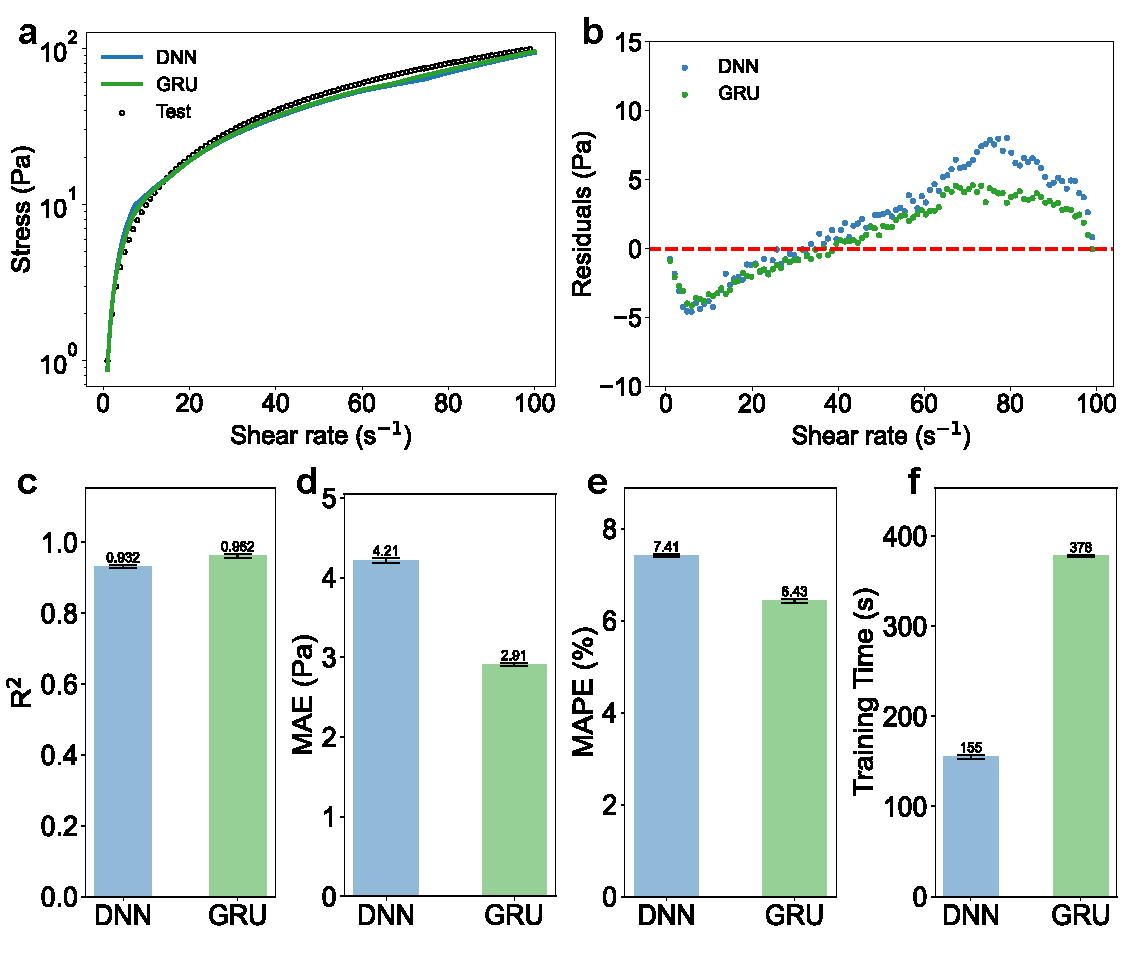
\includegraphics[width=0.8\textwidth]{Fig/Herschel_test.pdf}
  \FigureBicaption{\label{herschel_test}GRU算法和DNN算法在Herschel-Bulkley模型测试集上的预测效果对比示意图:(a)GRU和DNN在训练建模后的预测值-真实值曲线图;(b)GRU和DNN训练建模后的预测值残差图;(c)GRU和DNN测试集上的R$^2$指标图;(d)GRU和DNN在测试集上的MAE指标图;(e)GRU和DNN在测试集上的MAPE指标图;(f)GRU和DNN在测试集上的训练时间指标图}{Comparison schematic of the prediction performance of the GRU algorithm and the DNN algorithm on the Herschel-Bulkley model test set: (a) Predicted value–true value curves for GRU and DNN after training and modeling; (b) Residual plots of the predicted values for GRU and DNN after training and modeling; (c) R$^2$ metric plots on the test set for GRU and DNN; (d) MAE metric plots on the test set for GRU and DNN; (e) MAPE metric plots on the test set for GRU and DNN; (f) Training Time metric plots on the test set for GRU and DNN}
\end{figure}
\subsection{Maxwell模型建模}
\subsubsection{数值模拟数据}
\begin{figure}[htbp]
  \centering
  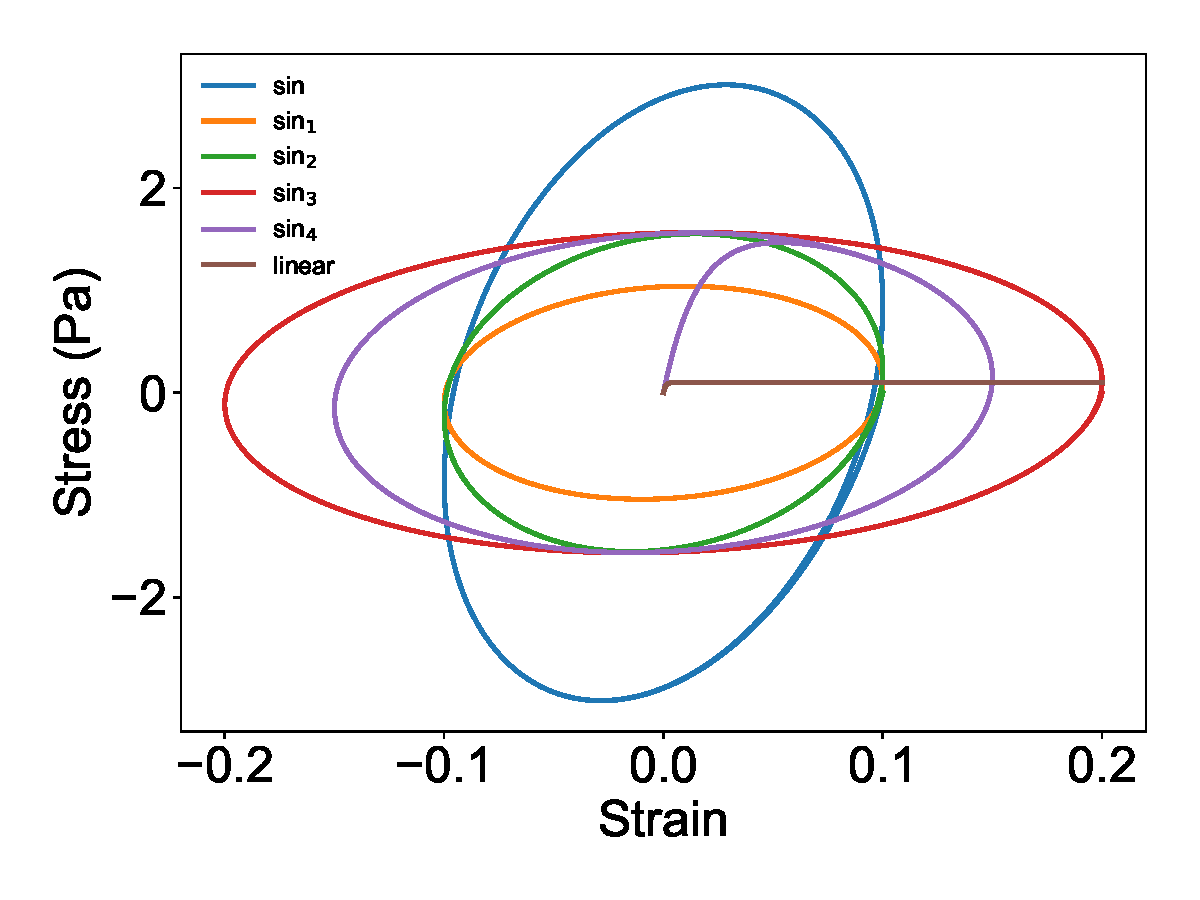
\includegraphics[width=0.8\textwidth]{Fig/maxwell_moni.pdf}
  \FigureBicaption{\label{maxwell_moni}不同应变变化协议的Maxwell模型模拟数据应力-应变曲线(Lissajous曲线)图}{Stress–strain curves (Lissajous curves) of simulated data for the Maxwell model under different strain variation protocols}
\end{figure}
本节通过后向欧拉法对简单 Maxwell 模型进行了数值模拟,生成了模拟数据,并绘制了应力-应变曲线(Lissajous 曲线),结果如图 \ref{maxwell_moni} 所示。图 \ref{maxwell_moni} 展示了不同应变协议下的模拟结果。对于正弦交变应变,Lissajous 曲线呈现出标准的闭合椭圆形状,这与 Maxwell 模型的理论预期一致,表明模型在周期性应变下的响应具有良好的稳定性和可预测性。对于线性应变,Lissajous 曲线在应变较小时表现出应力的快速增加,随后随着应变的继续增加,应力逐渐趋于一个稳定值,这一现象同样符合 Maxwell 模型的理论预期,反映了材料在持续应变下的应力松弛特性。综合看来,后向欧拉法模拟的数据符合预期,可以用于后续训练。


\subsubsection{交变协议预测交变协议效果验证}
\begin{figure}[htbp]
  \centering
  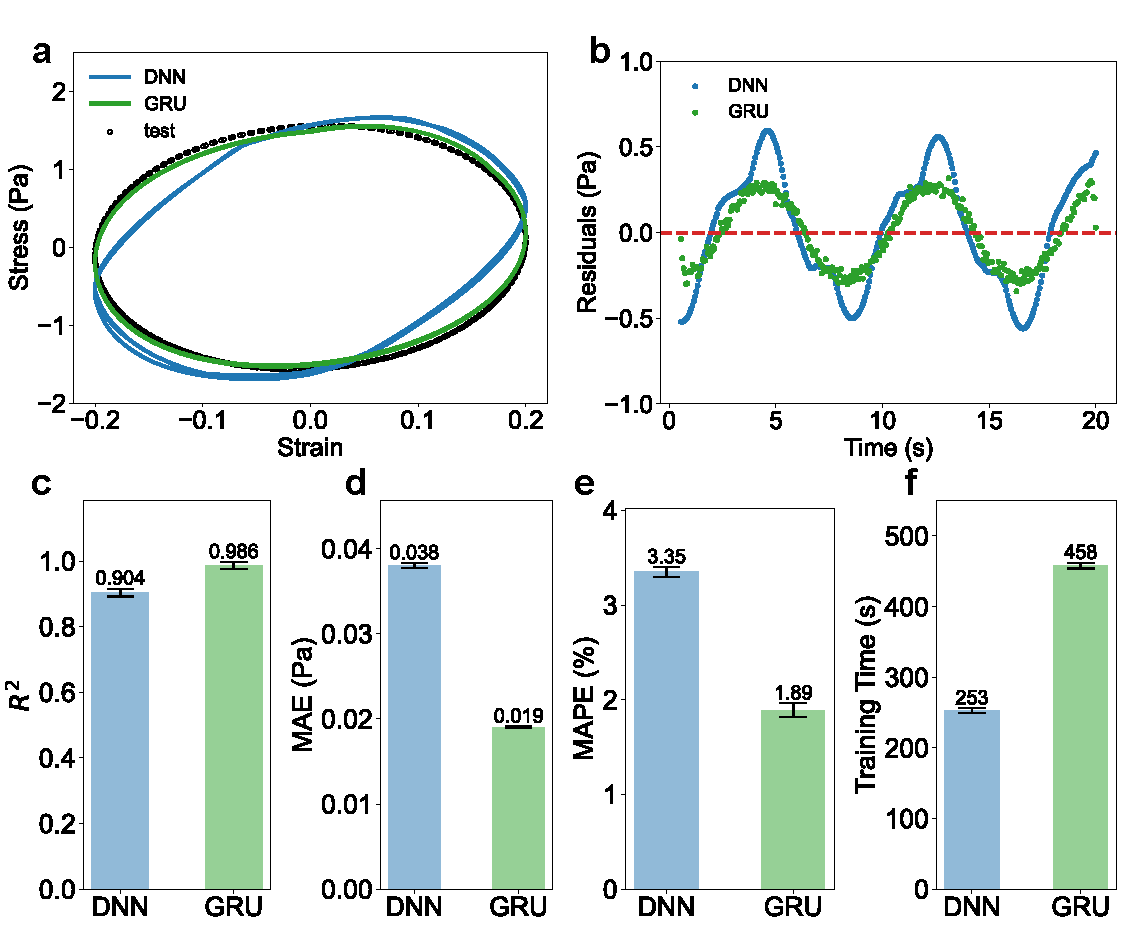
\includegraphics[width=0.8\textwidth]{Fig/Maxwell_sin_test.pdf}
  \FigureBicaption{\label{maxwell_sin}GRU算法和DNN算法在Maxwell模型交变协议测试集上的预测效果对比示意图:(a)GRU和DNN在测试集上的预测值与真实值的应力-应变曲线(Lissajous曲线);(b)GRU和DNN在测试集上的预测值与真实值的应力-时间曲线;(c)GRU和DNN在测试集上的预测值残差图}{Comparison of prediction performance between GRU and DNN algorithms on Maxwell model alternating protocol test set: (a) Stress-strain curves (Lissajous curves) of predicted vs. true values for GRU and DNN on test set; (b) Stress-time curves of predicted vs. true values for GRU and DNN on test set; (c) Residual plots of predicted values for GRU and DNN on test set}
\end{figure}
\begin{figure}[htbp]
  \centering
  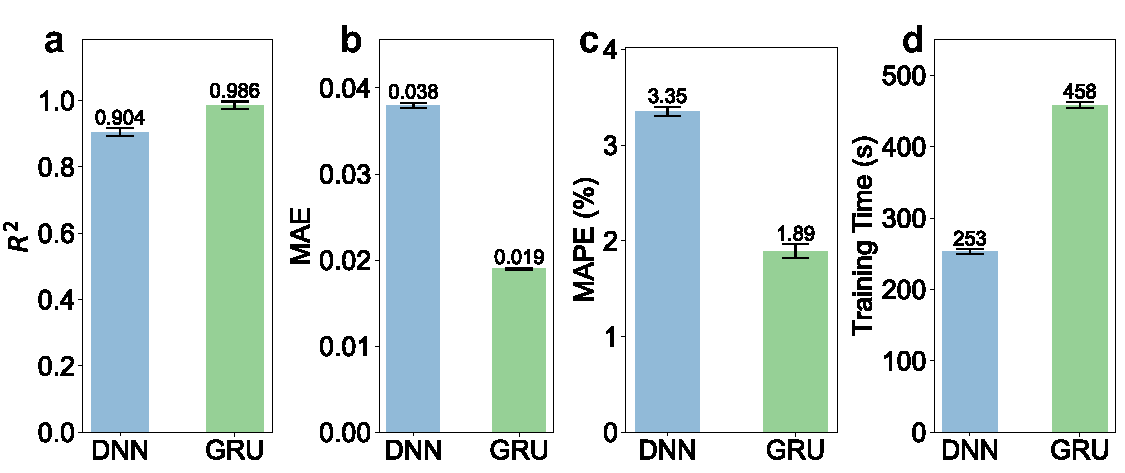
\includegraphics[width=0.8\textwidth]{Fig/Maxwell_sin_metric.pdf}
  \FigureBicaption{\label{maxwell_sin_metric}GRU算法和DNN算法在Maxwell模型交变测试集上的预测指标对比图:(a)GRU和DNN在测试集上的R$^2$指标图;(b)GRU和DNN在测试集上的MAE指标图;(c)GRU和DNN在测试集上的MAPE指标图;(d)GRU和DNN在测试集上的训练时间指标图}{Comparison schematic of the prediction performance of the GRU algorithm and the DNN algorithm on the Maxwell model alternating protocol test set: (a) R$^2$ metric plots on the test set for GRU and DNN; (b) MAE metric plots on the test set for GRU and DNN; (c) MAPE metric plots on the test set for GRU and DNN; (d) Training Time metric plots on the test set for GRU and DNN}
\end{figure}
为了验证GRU算法在时间序列本构方程数据中的预测效果,本节使用交变应变协议生成的数据作为训练集,交变应变协议生成的数据作为测试集。分别使用了GRU和DNN进行训练,并在测试集上进行验证,测试结果如图\ref{maxwell_sin}、图\ref{maxwell_sin_metric}所示。

图\ref{maxwell_sin}(a-b)为两种不同算法预测模型在测试集上的真实值-预测值曲线,
图a为Lissajous曲线,可以看到GRU算法的预测值的Lissajous曲线与真实值曲线十分接近,而DNN算法的预测值的Lissajous曲线与真实的曲线则有明显的周期性偏差,尤其在大应变时,预测值与真实值有较大的偏差。图b为时间-应力曲线,从中可以看到GRU算法的预测值曲线随时间变化较为稳定,贴近真实值曲线,而DNN算法的预测值的曲线明显偏离真实值曲线。

图\ref{maxwell_sin}(c)为两种算法预测模型的测试集残差图,从图中可以看到DNN算法的预测值与真实值残差呈现非常明显的周期性分布,极值偏离零刻度线,说明DNN模型无法泛化到测试集。而GRU的残差图虽然也存在一定周期性,但是总体分布效果明显优于DNN的对应残差,这说明GRU捕捉到了训练数据的较完整的特征,尤其是DNN未能捕捉的周期性特征。综合真实值-预测值曲线和残差图,可以定性分析出GRU的预测效果更为优秀。


接下来,本节计算两种算法的测试集预测指标,绘制指标对比图\ref{maxwell_sin_metric}。从图\ref{maxwell_sin_metric
}(a)显示,GRU的R$^2$值为0.986,接近1,说明GRU的预测效果十分优秀,而DNN的R$^2$值为0.904,略低于GRU,但是也高于0.9,属于非常出色的指标。仅从R$^2$指标来看,GRU预测效果优于DNN,但是优势不明显。从图\ref{maxwell_sin_metric}(b-c)看,GRU预测结果的MAE值为0.019,仅为DNN预测结果的MAE值的一半,GRU预测结果的MAPE值为1.89,仅为DNN预测结果的MAPE值3.35的一半。这定量说明GRU的预测结果误差远小于DNN的预测结果误差,GRU在此项任务上预测泛化效果更好。当然,由于GRU的模型特性,其训练时间如图\ref{maxwell_sin_metric}(d)所示,要高于DNN。

综合各项分析数据来看,当训练数据和测试数据为同类型应变变化过程(都为交变应变)时,GRU算法可以更好的学习到Maxwell模型数据的内在特征,包括周期性响应,黏弹性,时间依赖性响应。从定性与定量分析结果看,GRU算法的预测泛化效果在此项任务上明显优于DNN,在计算资源足够时,GRU算法相比DNN性能更佳。


\subsubsection{交变协议预测线性协议效果验证}
\begin{figure}[htbp]
  \centering
  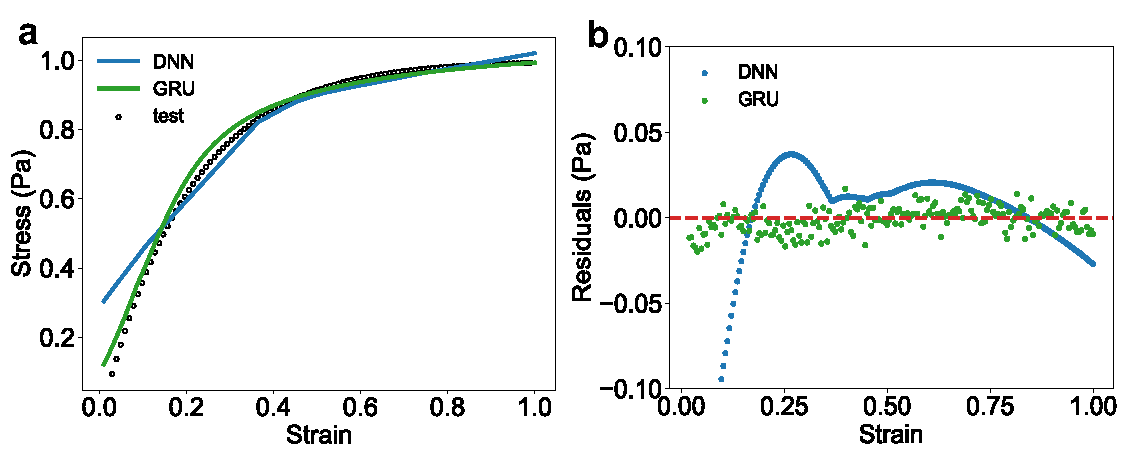
\includegraphics[width=0.8\textwidth]{Fig/maxwell_linear_test.pdf}
  \FigureBicaption{\label{maxwell_linear}GRU算法和DNN算法在Maxwell模型线性协议测试集上的预测效果对比示意图:(a)GRU和DNN在测试集上的预测值与真实值的应力-应变曲线(Lissajous曲线);(b)GRU和DNN在测试集上的预测值残差图}{Comparison of prediction performance between GRU and DNN algorithms on Maxwell model linear protocol test set: (a) Stress-strain curves (Lissajous curves) of predicted vs. true values for GRU and DNN on test set; (b) Residual plots of predicted values for GRU and DNN on test set}
\end{figure}
为了验证GRU算法在不同形式的应变历史下的泛化预测效果,本节使用交变应变协议生成的数据作为训练集,线性应变协议生成的数据作为测试集。分别使用了GRU和DNN进行训练,并在测试集上进行验证,测试结果如图\ref{maxwell_linear}、图\ref{maxwell_linear_metric}所示。
\begin{figure}[htbp]
  \centering
  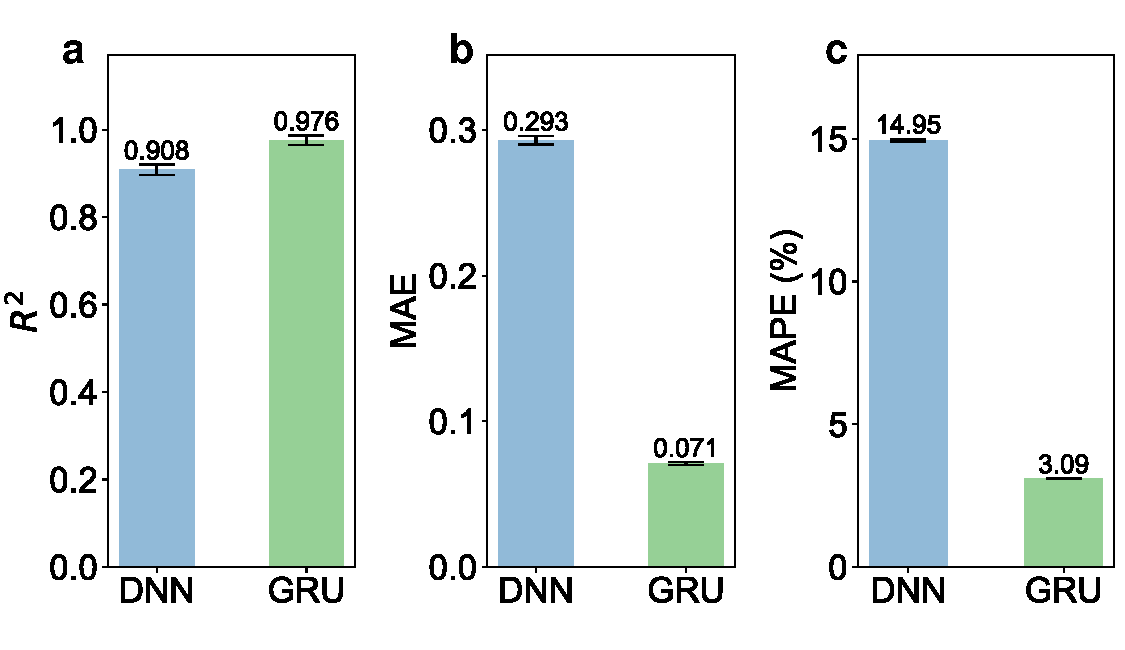
\includegraphics[width=0.8\textwidth]{Fig/maxwell_linear_metric.pdf}
  \FigureBicaption{\label{maxwell_linear_metric}GRU算法和DNN算法在Maxwell模型线性协议测试集上的预测指标对比图:(a)GRU和DNN在测试集上的R$^2$指标图;(b)GRU和DNN在测试集上的MAE指标图;(c)GRU和DNN在测试集上的MAPE指标图}{Comparison schematic of the prediction performance of the GRU algorithm and the DNN algorithm on the Maxwell model linear protocol test set: (a) R$^2$ metric plots on the test set for GRU and DNN; (b) MAE metric plots on the test set for GRU and DNN; (c) MAPE metric plots on the test set for GRU and DNN}
\end{figure}
图\ref{maxwell_linear}(a)为两种不同算法预测模型在测试集上的真实值-预测值的Lissajous曲线,图中可以看到GRU算法的预测值的Lissajous曲线与真实值曲线接近,在小应变时有一定偏差,这可能源于门控单元对初始状态记忆单元的权重初始化敏感性问题。而DNN算法的预测值的Lissajous曲线与真实的曲线相比GRU偏差更大,在小应变时,预测值与真实值有较大的偏差。

图\ref{maxwell_linear}(b)为两种算法预测模型的测试集残差图,从图中可以看到DNN算法的残差在初始时相比GRU更为偏离零刻度线,GRU的残差图残差点相对均匀地分布在零刻度线两侧,总体分布效果明显优于DNN的对应残差。这说明GRU捕捉到了训练数据的较完整的特征,且预测偏差较小。综合真实值-预测值曲线和残差图,可以定性分析出GRU的预测效果更为优秀。

接下来,本节计算两种算法的测试集预测指标,绘制指标对比图\ref{maxwell_linear_metric}。图\ref{maxwell_linear_metric}(a)显示,GRU的R$^2$值为0.976,接近1,证明GRU的预测效果十分优秀,而DNN的R$^2$值为0.908,略低于GRU,但是也高于0.9,属于非常出色的指标。仅从R$^2$指标来看,GRU预测效果优于DNN,但是优势不明显。从图\ref{maxwell_linear_metric}(b-c)看,GRU预测结果的MAE值为0.071,而DNN的预测结果的MAE值为0.293,GRU在绝对误差上仅为DNN的四分之一,优势显著。GRU预测结果的MAPE值为3.09,仅为DNN预测结果的MAPE值14.95的五分之一左右。这定量说明GRU的预测结果误差远小于DNN的预测结果误差,GRU在此项任务上预测泛化效果更好。这里的训练时间对比与上一节的交变协议预测交变协议一致,同图\ref{maxwell_sin_metric}(d)所示。


综合各项分析数据来看,当训练数据和测试数据为不同类型应变变化过程时,GRU算法展现出了显著的优势,尤其是在学习Maxwell模型数据的内在特征方面。Maxwell模型作为一种经典的粘弹性模型,其核心在于描述材料在应力作用下的时间依赖性响应。GRU算法可以仅通过学习交变应变的训练数据,就能够很好地预测线性应变的测试数据。这是因为GRU算法能够有效地从交变应变数据中提取出关键的时间依赖性特征,并将其应用于线性应变的预测中。
\subsubsection{不同时间步的预测效果对比}
\begin{figure}[htbp]
  \centering
  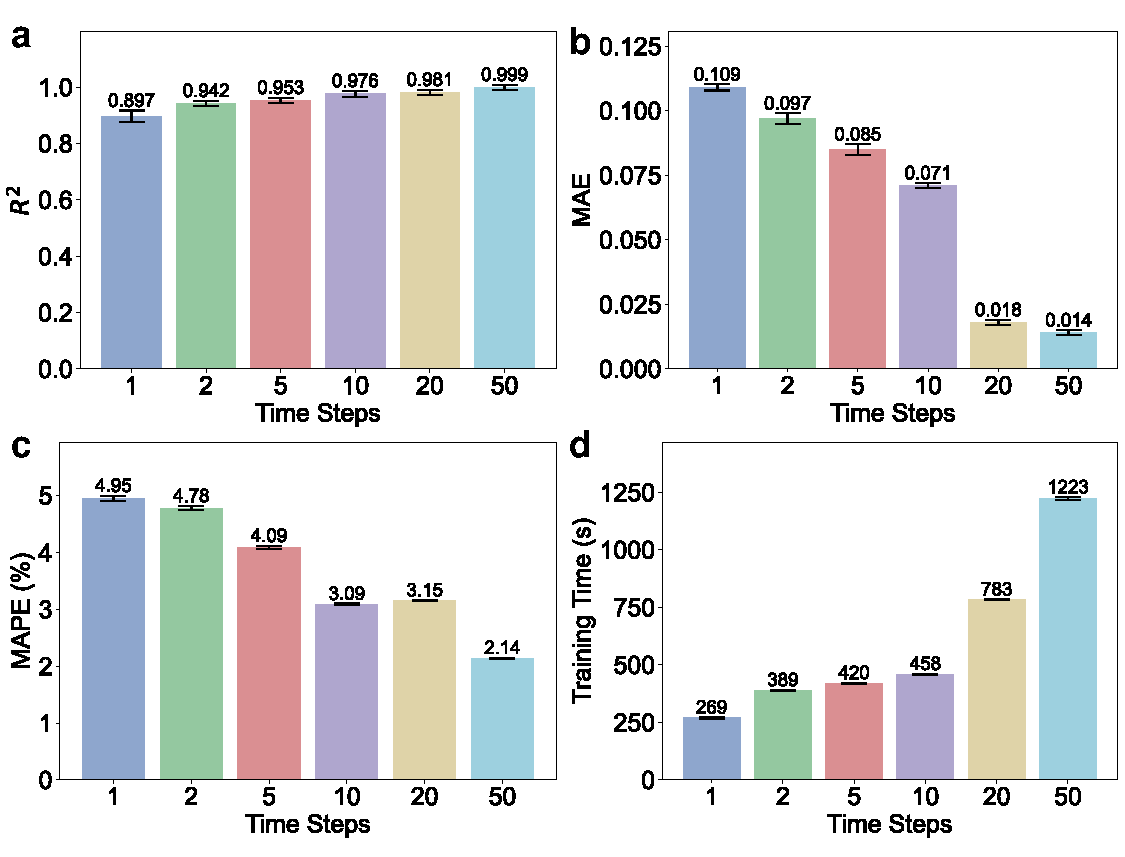
\includegraphics[width=0.8\textwidth]{Fig/Maxwell_timesteps_metrics.pdf}
  \FigureBicaption{\label{maxwell_timesteps_metrics}GRU算法在Maxwell模型不同时间步下的预测效果对比图:(a)GRU在不同时间步下的R$^2$指标图;(b)GRU在不同时间步下的MAE指标图;(c)GRU在不同时间步下的MAPE指标图;(d)GRU在不同时间步下的训练时间指标图}{Comparison of prediction performance of the GRU algorithm on the Maxwell model with different time steps: (a) R$^2$ metric plots with different time steps; (b) MAE metric plots with different time steps; (c) MAPE metric plots with different time steps; (d) Training Time metric plots with different time steps}
\end{figure}
对于GRU这类循环神经网络来说,网络架构的时间步数(序列长度)是非常重要的超参数。较大的时间步可以使模型在每个时间步上处理更多的信息,有助于捕捉长期依赖关系,但是可能导致模型学习到数据中的噪声,而不是其潜在的结构,从而导致过拟合。较小的时间步较小的时间步可以更细致地捕捉序列中的短期变化和细节信息,有助于模型更好地理解数据的短期动态特征,可能导致模型过于关注噪声,而忽略重要的长期依赖关系,从而导致欠拟合。本节研究了不同时间步下训练的模型在测试集上的预测效果。如图\ref{maxwell_timesteps_metrics}所示。由图可见,预测模型R$^2$值随着时间步的增加而增加,但是幅度较小。MAE值和MAPE值随时间步的增加而减少,说明随着时间步的增加,模型的预测效果变的更好,时间步小于10时,这种误差减小的趋势较明显,时间步大于20时,MAE值下降幅度变小,时间步大于10,MAPE值下降幅度变小。这说明模型的优化指标上升存在阈值,这是因为GRU算法在较长序列中容易遗忘丢失信息,对于时间序列的处理长度有一定限制。而随着时间步的增加,当时间步大于20后,模型的训练时间急剧增加,训练成本陡增。

本节分析针对此项任务,最佳时间步在10-20之间,MAE值和MAPE值开始下降到阈值,且训练时间还未显著增加。


% Doi-Edwards模型建模
\subsection{Doi-Edwards模型建模}
\subsubsection{数值模拟数据}
\begin{figure}[htbp]
  \centering
  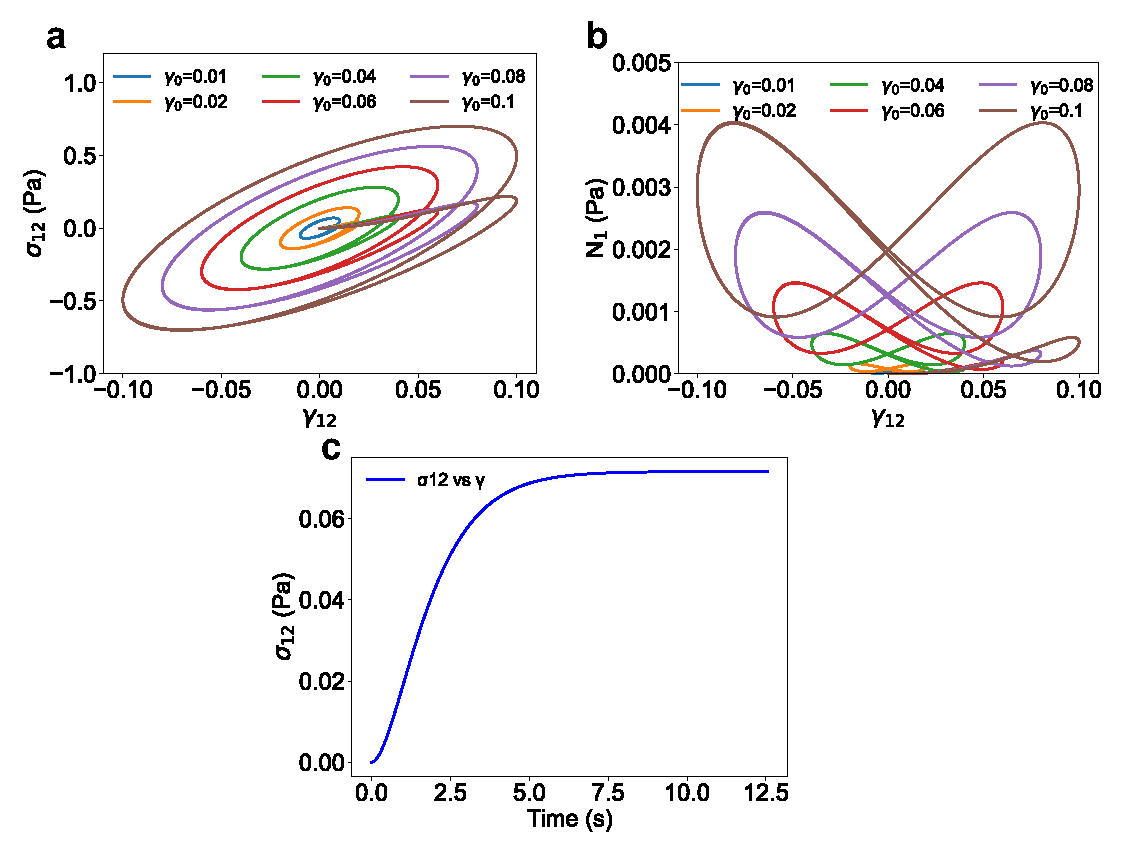
\includegraphics[width=0.8\textwidth]{Fig/doi-edwards-moni.pdf}
  \FigureBicaption{\label{doi-edwards-moni}Doi-Edwards模型模拟数据:(a)不同应变振幅下的剪切应力应变Lissajous曲线;(b)不同应变振幅下的第一法向应力差($N_1$)的Lissajous曲线;(c)线性应变协议下的应力-时间曲线}{Doi-Edwards model simulation data: (a) Lissajous curves of shear stress-strain under different strain amplitudes; (b) Lissajous curves of first normal stress difference ($N_1$); (c) Stress-time curves under linear strain protocol}
\end{figure}
本节使用Python的scipy.integrate库对Doi-Edwards模型进行数值积分模拟。模拟结果如图\ref{doi-edwards-moni}所示。图\ref{doi-edwards-moni}(a)为不同应变振幅模拟的剪切应力应变Lissajous曲线,曲线呈现标准的椭圆形状,符合Doi-Edwards模型在小应变下的假设。图\ref{doi-edwards-moni}(b)为模拟的第一法向应力差($N_1$)的Lissajous曲线,曲线具有振幅依赖性,且为滞回曲线,与文献中的Doi-Edwards模型一致。图\ref{doi-edwards-moni}(c)为线性应变协议下的应力-时间曲线,可以看到随着应变加载,应力一开始为近似的线性增加,后逐渐趋向平台值,这个结果符合预期。综上本节模拟的数据可以认为符合Doi-Edwards模型,可以用于后续实验。

\subsubsection{交变协议预测交变协议效果验证}
\begin{figure}[htbp]
  \centering
  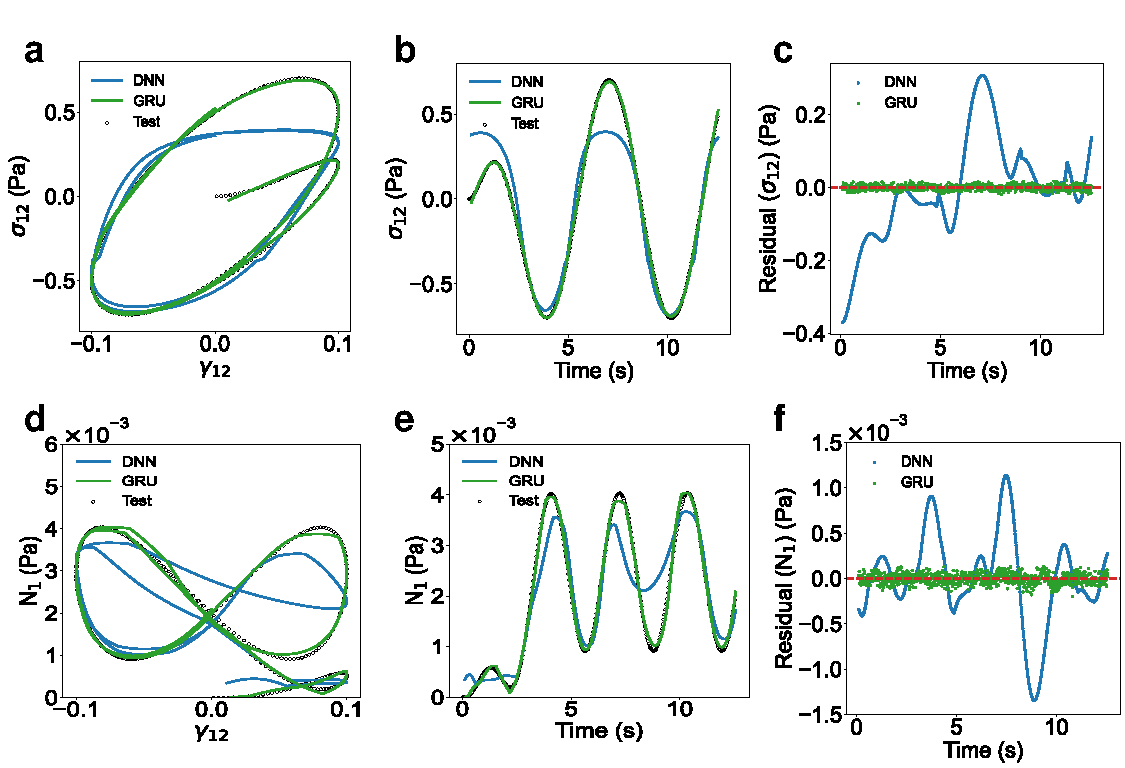
\includegraphics[width=0.8\textwidth]{Fig/doi-edwards-sin.pdf}
  \FigureBicaption{\label{doi-edwards-sin}GRU算法和DNN算法在Doi-Edwards模型交变协议测试集上的预测效果对比示意图:(a)GRU和DNN在测试集上的预测值与真实值的剪切应力-应变曲线(Lissajous曲线);(b)GRU和DNN在测试集上的预测值与真实值的时间-应力曲线;(c)GRU和DNN在测试集上剪切应力的预测值残差图;(d)GRU和DNN在测试集上的预测值与真实值的第一法向应力差($N_1$)的Lissajous曲线;(e)GRU和DNN在测试集上的预测值与真实值的时间-第一法向应力差曲线;(f)GRU和DNN在测试集上的第一法向应力差预测值残差图}{Comparison schematic of the prediction performance of the GRU algorithm and the DNN algorithm on the Doi-Edwards model alternating protocol test set: (a) Shear stress-strain curves (Lissajous curves) of predicted vs. true values for GRU and DNN on test set; (b) Time-stress curves of predicted vs. true values for GRU and DNN on test set; (c) Residual plots of shear stress predicted values for GRU and DNN on test set; (d) First normal stress difference ($N_1$) Lissajous curves of predicted vs. true values for GRU and DNN on test set; (e) Time-first normal stress difference curves of predicted vs. true values for GRU and DNN on test set; (f) Residual plots of first normal stress difference predicted values for GRU and DNN on test set}
\end{figure}
\begin{figure}[htbp]
  \centering
  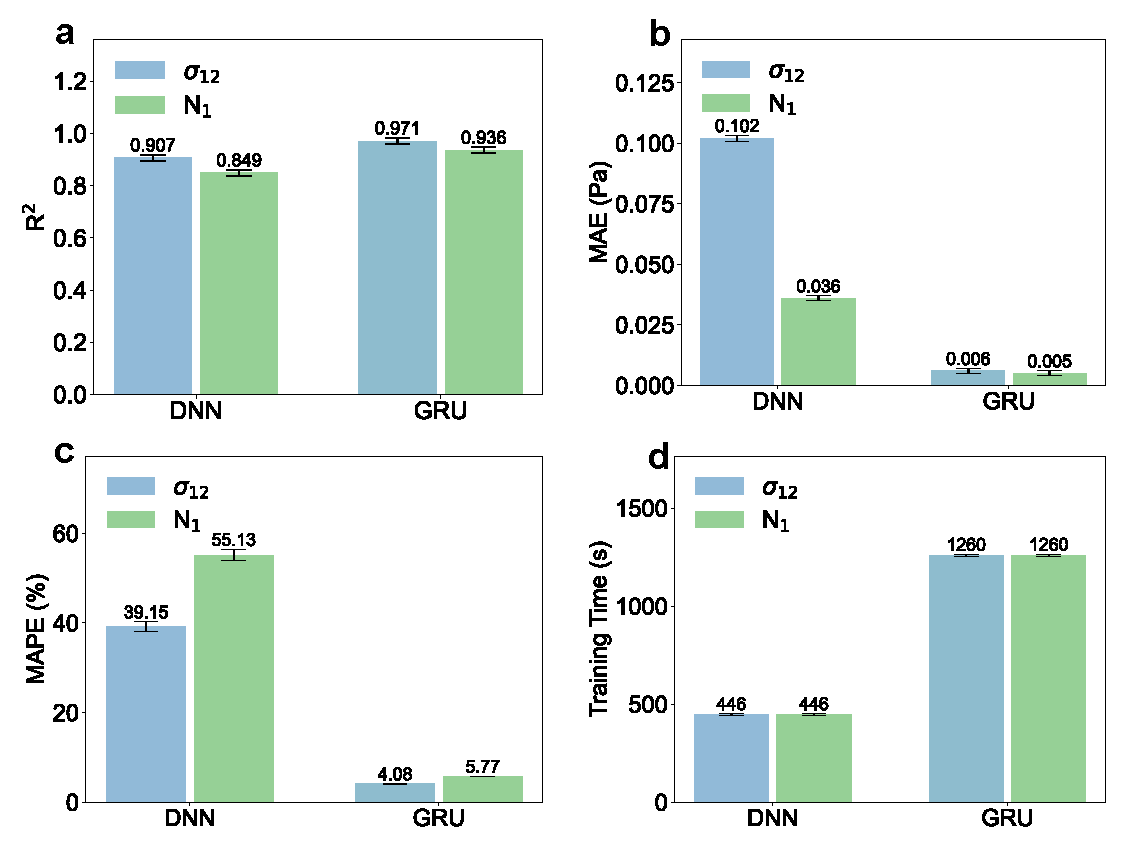
\includegraphics[width=0.8\textwidth]{Fig/doi-edwards-sin-metrics.pdf}
  \FigureBicaption{\label{doi-edwards-sin-metric}GRU算法和DNN算法在Doi-Edwards模型交变协议测试集上的预测指标对比图:(a)GRU和DNN在测试集上的R$^2$指标图;(b)GRU和DNN在测试集上的MAE指标图;(c)GRU和DNN在测试集上的MAPE指标图;(d)GRU和DNN在测试集上的训练时间指标图}{Comparison schematic of the prediction performance of the GRU algorithm and the DNN algorithm on the Doi-Edwards model alternating protocol test set: (a) R$^2$ metric plots on the test set for GRU and DNN; (b) MAE metric plots on the test set for GRU and DNN; (c) MAPE metric plots on the test set for GRU and DNN; (d) Training Time metric plots on the test set for GRU and DNN}
\end{figure}
为了验证GRU算法在Doi-Edwards模型本构方程数据中的预测效果,本节使用交变应变协议生成的数据作为训练集,交变应变协议生成的数据作为测试集。分别使用了GRU和DNN进行训练,并在测试集上进行验证,测试结果如图\ref{doi-edwards-sin}、图\ref{doi-edwards-sin-metric}所示。

图\ref{doi-edwards-sin}(a-c)为两种不同算法构建的预测模型预测的剪切应力($\sigma_{12}$)的Lissajous曲线、时间-应力曲线、残差图,(d-f)为预测的第一法向应力差($N_1$)的Lissajous曲线、时间-应力曲线、残差图。
图a和图b可以看出GRU算法的预测的$\sigma_{12}$值与真实的$\sigma_{12}$接近,曲线拟合较好。而DNN算法的预测值在某些区域存在较大误差,例如在应变变化的初始和$5\sim10$ s之间,DNN存在较大误差。图c的残差图则显示,GRU算法预测值与真实值的残差紧贴零刻度线,呈现无序离散的分布状态,而DNN算法预测值和真实值的残差呈现明显的曲线规律,且与零刻度线性距离偏差较大,残差分布区间远远大于GRU部分。残差图的结果表明对于GRU成功地学习到了训练数据中的各项特征,复杂的非线性关系,且不存在明显周期性,总体残差较小,而DNN存在特征未能完全学习的问题,拟合效果较差,未能很好地捕捉到训练数据的特征。从图d、图e和图f的$N_1$的预测效果图来看,$N_1$与$\sigma_{12}$的结果类似,均是GRU的预测效果要由于DNN,而对比GRU预测的$N_1$值和$\sigma_{12}$值,则是$\sigma_{12}$值的预测效果会更好,这可能是因为$\sigma_{12}$与输入的剪切速率特征$\dot{\gamma_{12}}$之间的函数关系更为简单,且更加符合时间叠加原理,所以GRU可以更好地捕捉其时间依赖性和内在联系。


之后本节分别对两种不同算法在$\sigma_{12}$和$N_1$上的预测效果做了定量分析,指标图如图\ref{doi-edwards-sin-metric}所示。在R$^2$指标上,GRU在$\sigma_{12}$和$N_1$的预测指标均优于DNN,而同种算法下$\sigma_{12}$的R$^2$值要高于$N_1$,显示$\sigma_{12}$的预测效果更好。在MAE指标上,DNN的$\sigma_{12}$和$N_1$的MAE值均远高于GRU,说明GRU的预测误差远小于DNN。MAPE指标与MAE指标的对比基本一致,都是GRU的预测误差小于DNN。但是同种算法下$\sigma_{12}$的MAE值高于$N_1$,但是MAPE值反之,这是因为MAE值强调的是绝对值比较,受到真实数据本身尺度的影响,因此比较同种算法下$\sigma_{12}$和$N_1$的预测效果应当以去除了数据尺度影响的MAPE值来判定,而MAPE值的结论表明同种算法下$\sigma_{12}$值的预测效果相比$N_1$更好,这与R$^2$的分析和图\ref{doi-edwards-sin}的定性分析一致,这也是后续可以优化的方向之一。最后,从图\ref{doi-edwards-sin-metric}(d)来看,GRU在此项任务上的训练时间为DNN的3倍左右,符合更高成本的预期。

综合各项分析数据来看,当训练数据和测试数据为同类型应变变化过程(都为交变应变)时,GRU算法可以更好的学习到Doi-Edwards模型数据的内在特征,包括周期性响应,黏弹性,时间依赖性响应。从定性与定量分析结果看,GRU算法的预测泛化效果在此项任务上明显优于DNN,在计算资源足够时,GRU算法相比DNN性能更佳,而在同种算法下$\sigma_{12}$的预测效果优于$N_1$。
\subsubsection{交变协议预测线性协议效果验证}
\begin{figure}[htbp]
  \centering
  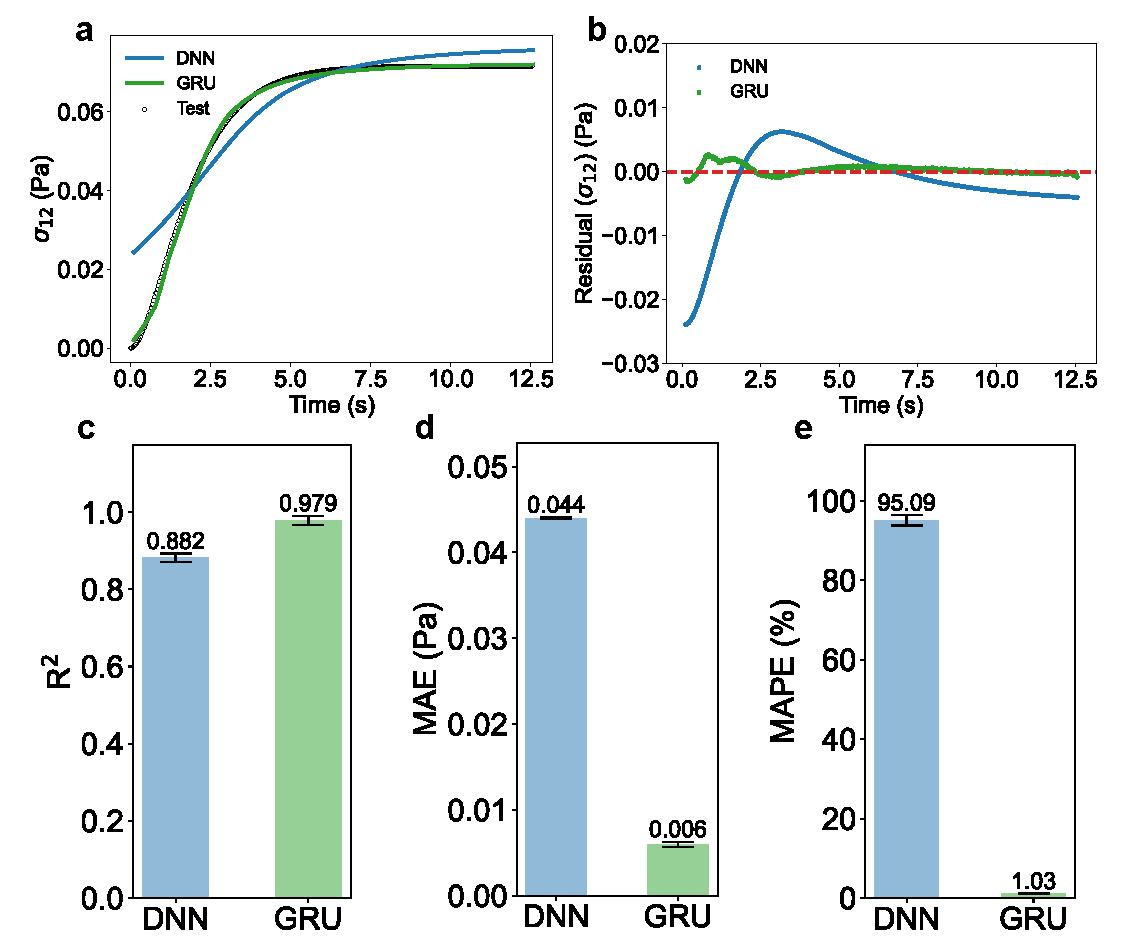
\includegraphics[width=0.8\textwidth]{Fig/doi-edwards-linear.pdf}
  \FigureBicaption{\label{doi-edwards-linear}GRU算法和DNN算法在Doi-Edwards模型线性协议测试集上的预测效果对比示意图:(a)GRU和DNN在测试集上的预测值与真实值的剪切应力-应变曲线(Lissajous曲线);(b)GRU和DNN在测试集上的预测值残差图}{Comparison schematic of the prediction performance of the GRU algorithm and the DNN algorithm on the Doi-Edwards model linear protocol test set: (a) Shear stress-strain curves (Lissajous curves) of predicted vs. true values for GRU and DNN on test set; (b) Residual plots of predicted values for GRU and DNN on test set}
\end{figure}
\begin{figure}[htbp]
  \centering
  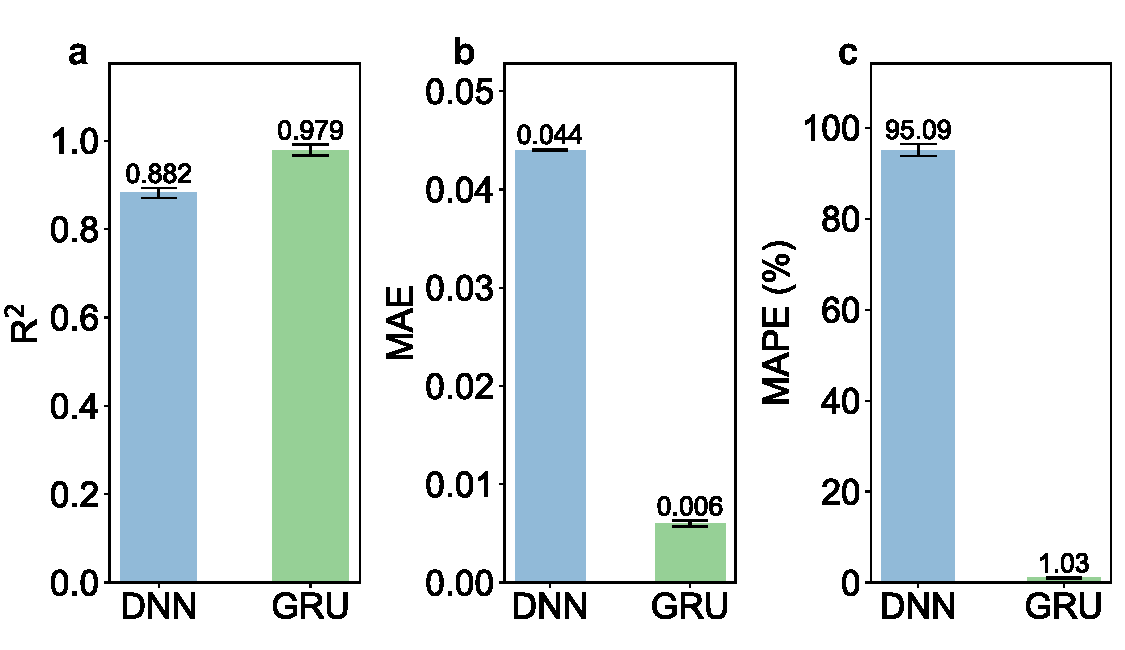
\includegraphics[width=0.8\textwidth]{Fig/doi-edwards-linear-metrics.pdf}
  \FigureBicaption{\label{doi-edwards-linear-metrics}GRU算法和DNN算法在Doi-Edwards模型线性协议测试集上的预测效果对比示意图:(a)GRU和DNN在测试集上的R$^2$指标图;(b)GRU和DNN在测试集上的MAE指标图;(c)GRU和DNN在测试集上的MAPE指标图}{Comparison schematic of the prediction performance of the GRU algorithm and the DNN algorithm on the Doi-Edwards model linear protocol test set: (a) R$^2$ metric plots on the test set for GRU and DNN; (b) MAE metric plots on the test set for GRU and DNN; (c) MAPE metric plots on the test set for GRU and DNN}
\end{figure}
为了验证GRU算法在不同形式的应变历史下对于Doi-Edwards模型泛化预测效果,本节使用交变应变协议生成的数据作为训练集,线性应变协议生成的数据作为测试集。分别使用了GRU和DNN进行训练,并在测试集上进行验证,测试结果如图\ref{doi-edwards-linear}、图\ref{doi-edwards-linear-metrics}所示。

图\ref{doi-edwards-linear}(a)为两种不同算法预测模型在测试集上的真实值-预测值曲线,图中可以看到GRU算法的预测值的曲线与真实值曲线接近,无较明显的偏差区间,而DNN算法的预测值的曲线与真实的曲线存在明显的偏差。在应变加载初始和结束时,DNN算法的预测值相比真实值偏大,而应变加载$2\sim6$ s的中间阶段,DNN算法的预测值又偏小,总体来看仅在大致趋势上符合真实值曲线。

图\ref{doi-edwards-linear}(b)展示了两种算法在测试集上的残差图。从图中可以明显看出,DNN算法的预测值与真实值之间的残差分布并不均匀,整体呈现出较为清晰的曲线趋势,尤其是在第3 s附近出现了显著的峰值。这表明DNN未能充分捕捉到训练数据中的关键特征,导致其在测试集上的表现不佳。相比之下,GRU算法的残差图则呈现出无序分布,残差点均匀地分布在零刻度线两侧,且残差值普遍小于DNN。这说明GRU能够更好地捕捉到训练数据中的特征,预测偏差也更小。综合真实值与预测值的曲线以及残差图的分析,可以定性地得出结论:GRU的预测效果优于DNN。

接下来,本节对两种算法在测试集上的预测性能指标进行了详细计算,并绘制了相应的指标对比图,如图\ref{doi-edwards-linear-metrics}所示。从图\ref{doi-edwards-linear-metrics}(a)中可以看出,GRU算法的 R$^2$值达到了0.979,这一结果充分证明了GRU在预测任务中的卓越表现。相比之下,DNN算法的 R$^2$值仅为0.882,明显低于GRU,这表明在 R$^2$指标的评估中,GRU的表现更为出色。进一步观察图\ref{doi-edwards-linear-metrics}(b-c),可以发现GRU预测结果的MAE值为0.006,而DNN的MAE值则高达0.044。这意味着GRU在绝对误差方面的表现仅为DNN的七分之一,优势极为显著。此外,GRU预测结果的MAPE值为1.03,而DNN的MAPE值则为95.09。这些定量数据充分说明了GRU的预测结果误差远小于DNN,从而证明了GRU在该任务上的预测泛化能力更强。
至于训练时间的对比,与上一节中交变协议预测交变协议的情况一致,具体可参考图\ref{doi-edwards-sin-metric}(d)所示。

从整体分析数据来看,当训练数据与测试数据涉及不同类型的应变变化过程时,GRU算法在学习Doi-Edwards模型数据的内在特性方面有显著优势。这主要归因于GRU算法能够高效地从交变应变数据中提取关键的时间依赖特征,并将其成功应用于线性应变的预测之中。

\subsubsection{不同时间步的预测效果对比}

为了探究在Doi-Edwards模型上GRU算法的最佳时间步,本节研究了不同时间步下训练的模型在测试集上的预测效果,如图\ref{doi-edwards-timesteps-metrics}所示。由图可见,预测模型R$^2$值在时间步小于40时随着时间步的增加而增加,在时间步大于40后反而略有下降。MAE值和MAPE值在时间步小于40时随时间步的增加而减少,时间步为40的值只有不到时间步为20的值的十分之一,显著下降,而时间步大于40后,MAE值和MAPE值则趋于稳定。这说明对于本项任务,时间步为40左右时,恰好可以开始获得不错的预测效果,而从训练成本来看,训练时间是随着时间步设置增加而单调增的,所以综合看来,时间步为40左右时,性价比最高。
\begin{figure}[H]
  \centering
  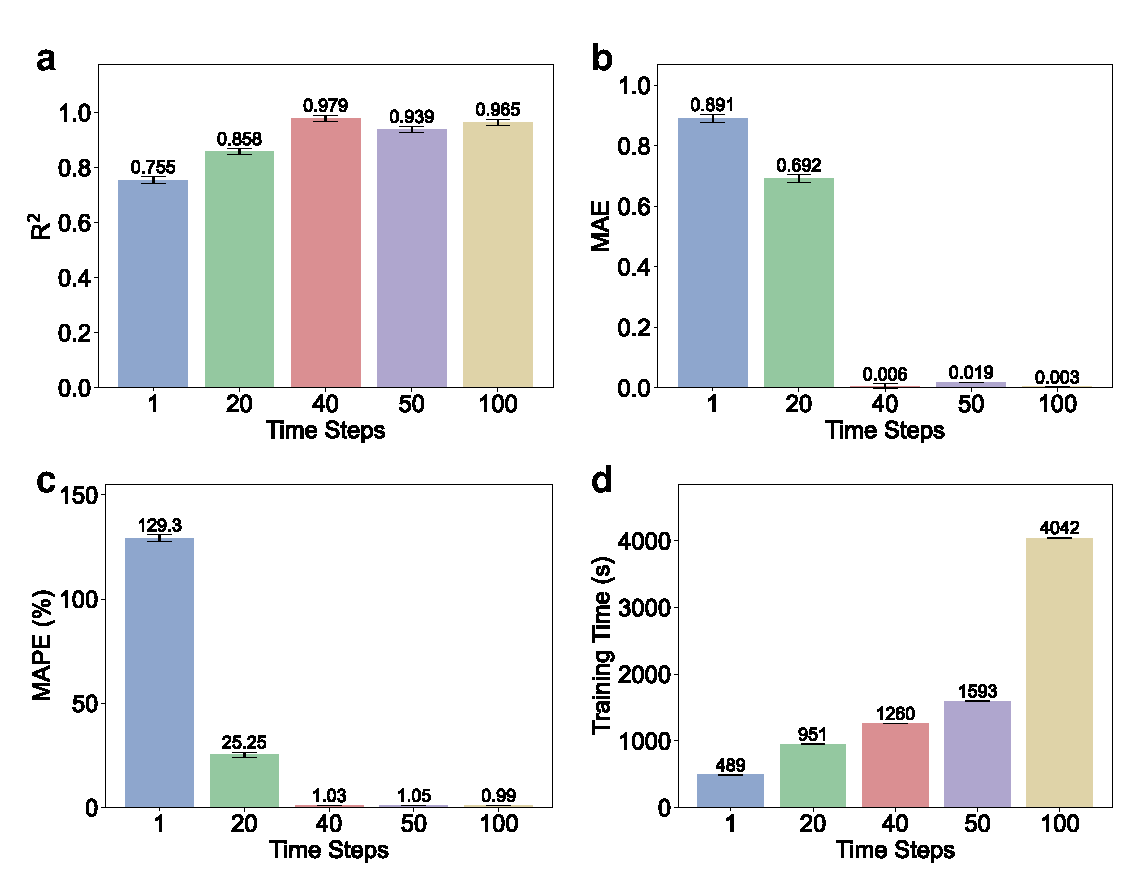
\includegraphics[width=0.8\textwidth]{Fig/doi-edwards-timesteps-metrics.pdf}
  \FigureBicaption{\label{doi-edwards-timesteps-metrics}GRU算法和DNN算法在Doi-Edwards模型不同时间步长下的预测指标对比图:(a)GRU和DNN在不同时间步下的R$^2$指标图;(b)GRU和DNN在不同时间步下的MAE指标图;(c)GRU和DNN在不同时间步下的MAPE指标图;(d)GRU和DNN在不同时间步下的训练时间指标图}{Comparison schematic of the prediction performance of the GRU algorithm and the DNN algorithm under different time steps of the Doi-Edwards model: (a) R$^2$ metric plots under different time steps for GRU and DNN; (b) MAE metric plots under different time steps for GRU and DNN; (c) MAPE metric plots under different time steps for GRU and DNN; (d) Training Time metric plots under different time steps for GRU and DNN}
\end{figure}




% 本章小结 
\section{本章小结}

本章首先运用了GRU算法对数值模拟的 Herschel-Bulkley 模型、Maxwell 模型以及Doi-Edwards 模型所产生的模拟数据展开深度学习建模工作。

研究结果揭示出,GRU 作为一种循环神经网络,依托其独特的门控单元机制,能够精准地捕捉黏弹性材料流变学模拟数据所蕴含的时间依赖性以及复杂非线性特征。特别的,在处理 Herschel-Bulkley 模型这类非时间序列数据时,GRU 模型的预测效果相较于DNN模型依旧略胜一筹。究其原因,在于 GRU 的门控单元机制引入了更多的参数,从而赋予了其更佳的泛化性能。对于经典的简单 Maxwell模型,由于属于典型的时间序列数据,GRU对其进行建模预测的效果全面超越DNN,各项评估指标均展现出显著优势。当面对更为复杂Doi-Edwards 模型时,GRU的建模预测效果依旧优于 DNN。进一步分析发现,在相同的建模任务中,GRU 在剪切应力$\sigma_{12}$的预测效果上强于第一法向应力差$N_1$。

在本章模拟数据预测部分设计的实验中,我们探讨了两类预测任务:首先,利用交变应变变化的训练数据,预测相应的测试数据;其次,使用交变应变变化实验的训练数据,预测稳态剪切的测试数据。在针对不同本构模型的这两类实验中,GRU模型的表现均优于DNN。这一现象充分表明,GRU具备更强的泛化能力,能够有效地预测更为一般化的本构关系,而不仅仅是进行简单的函数逼近。GRU通过引入门控机制,能够有效捕捉序列数据中的长期依赖关系,从而在处理复杂的本构模型时展现出更优的性能。相比之下,DNN虽然在非时序本构模型中表现出色,但在处理具有复杂时序特征的本构模型时,其性能会受到限制。因此,选择GRU模型进行本构关系的预测,能够更好地适应数据的复杂性和多样性,提升预测的准确性和可靠性,但是本章的实验结果同样表明,GRU模型由于其架构特征,比普通DNN的训练时间高很多,且训练时消耗更多的计算机资源(计算机内存、GPU显存等)。

综上所述,本章的研究工作充分验证了GRU在流变学数据建模中的优异效果。该模型不仅能够准确捕捉黏弹性材料的时间依赖性,从而高效刻画非线性、时变的物理过程,展现出良好的关联适配性,而且在理论上突破了传统数据拟合方法的局限,在模拟数据和真实实验数据中均表现出卓越的泛化能力和预测稳定性。总的来说,本章的研究为深度学习在流变学本构建模领域的应用开辟了全新的思路,即可以从模型升级的角度去优化本构建模的过程。





